\chapter{Software Architecture}\label{software_architecture}

\begin{figure}[h]
       \centering
       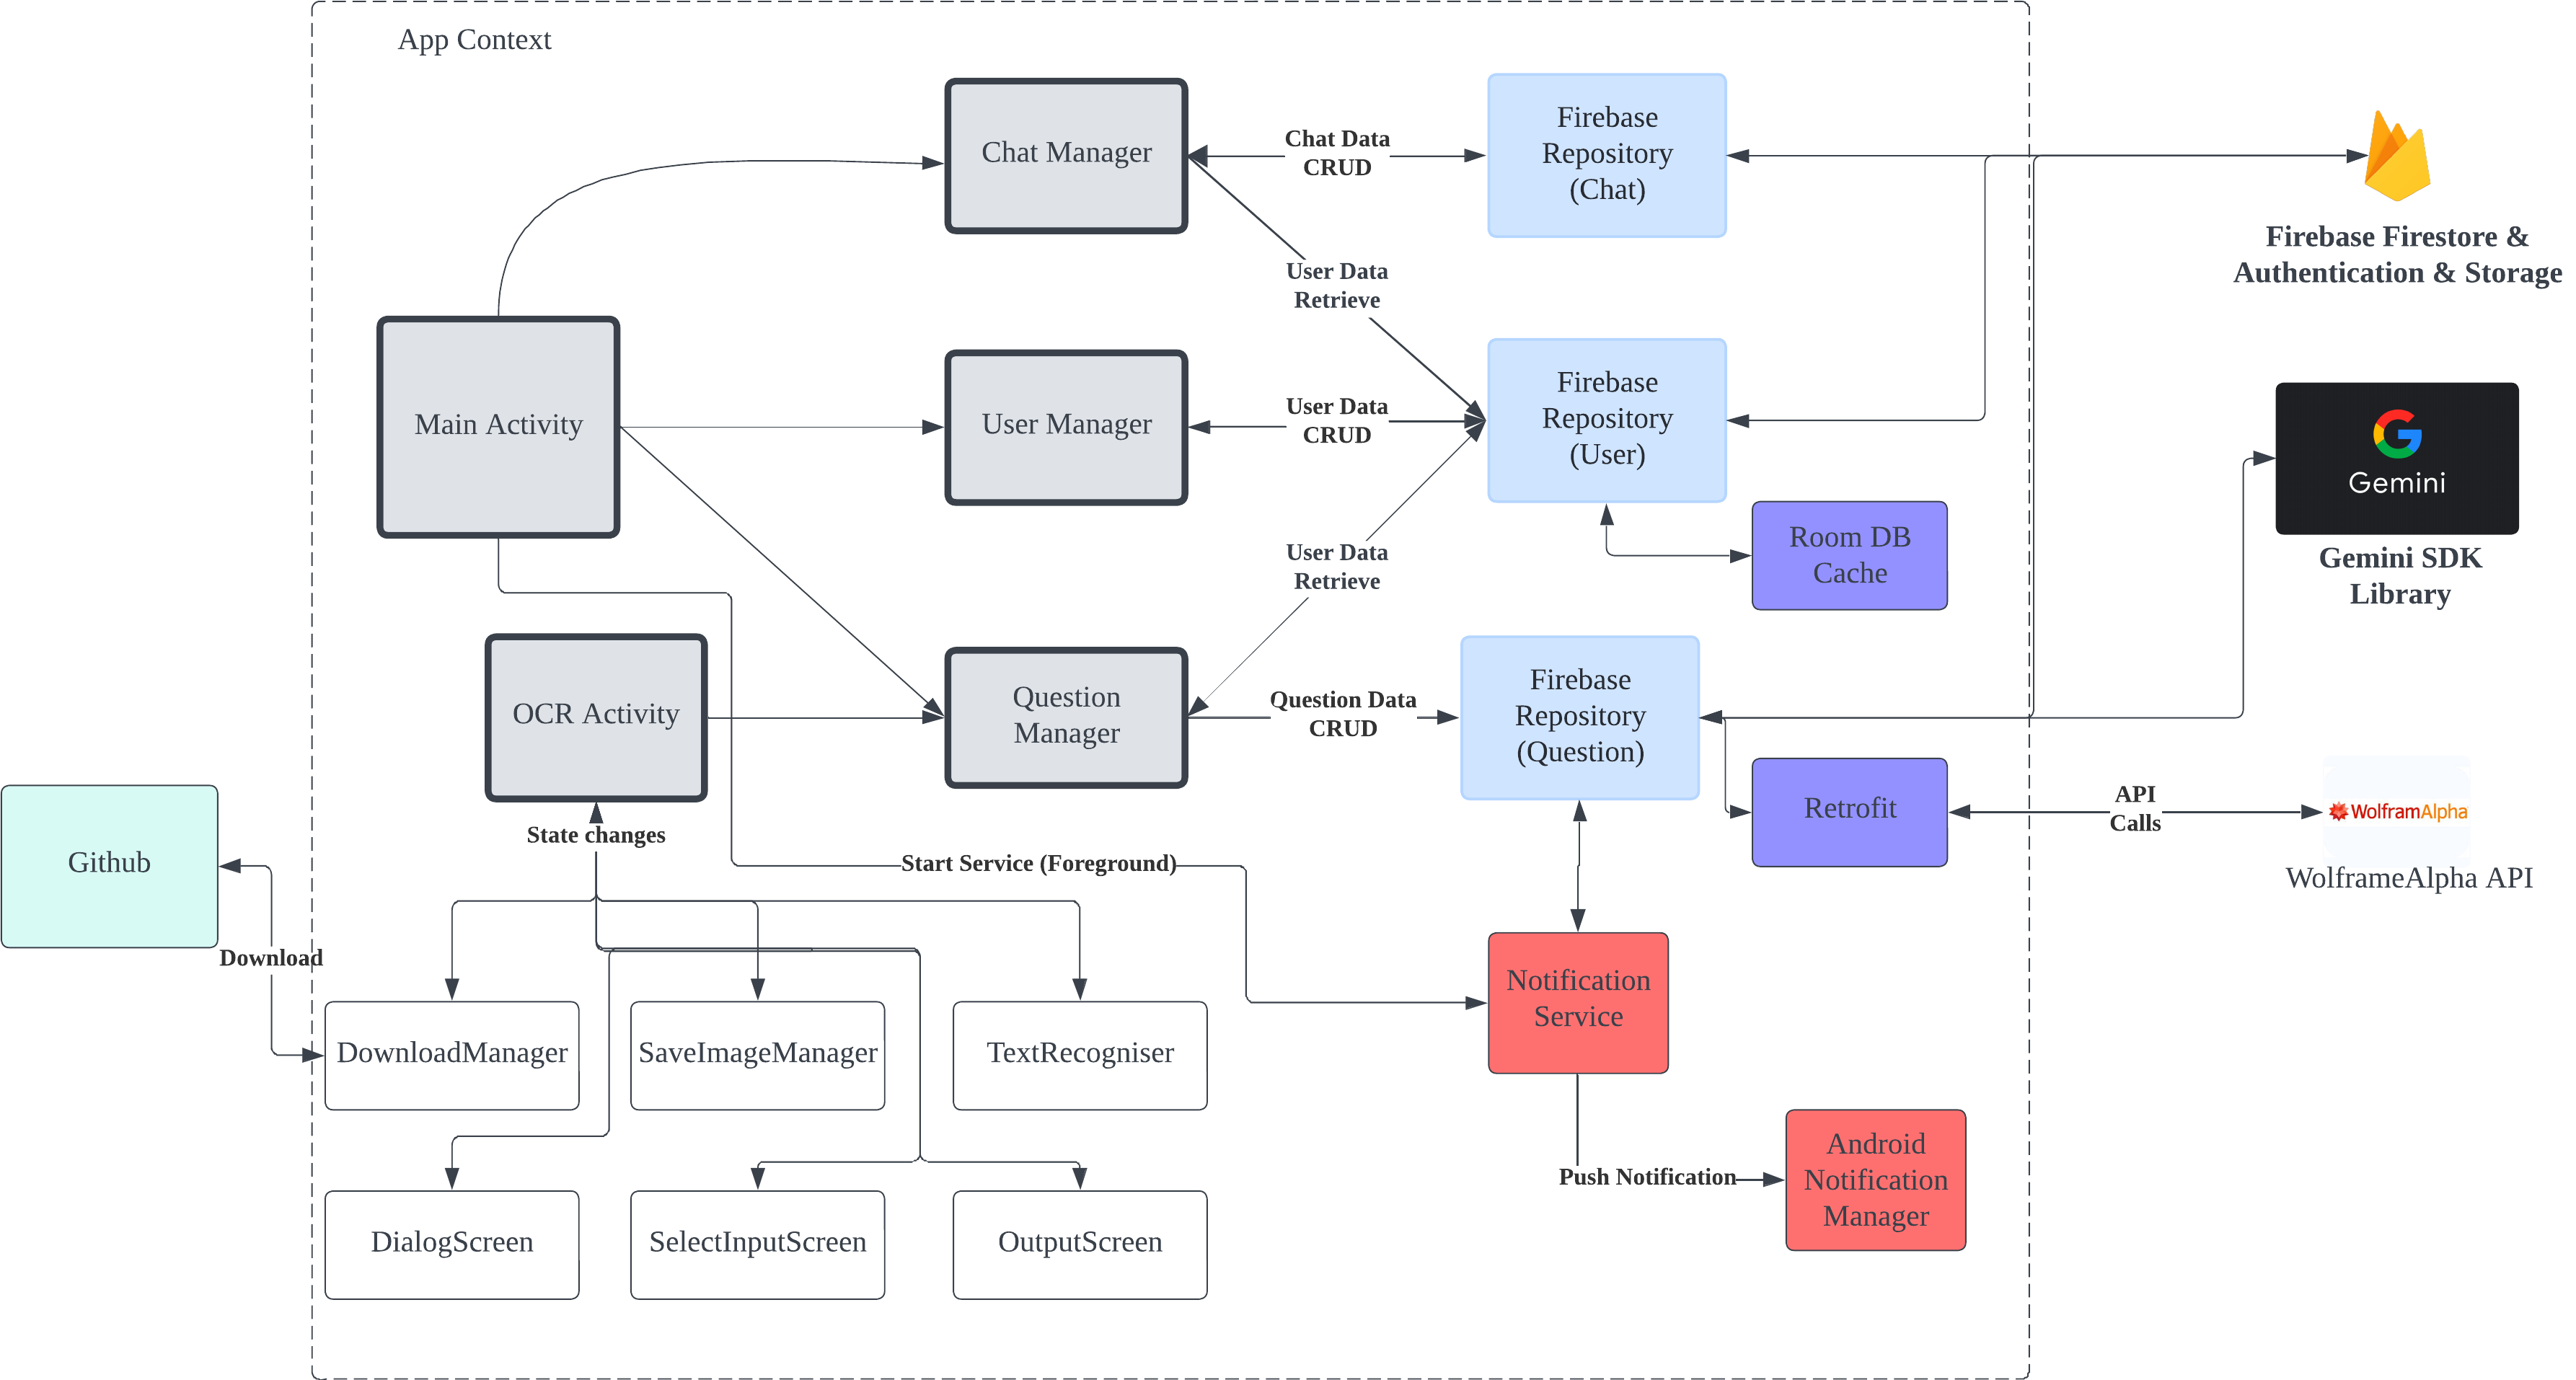
\includegraphics[scale = .20]{Figures/StudyTogether_Architecture.png}
       \caption{\footnotesize Initial Software Architecture}
       \label{StudyTogether_Architecture}
\end{figure}

The software architecture of our Android application, "Study Together," is depicted in the diagram. Our application makes extensive use of Firebase SDK for Authentication and Database services. Additionally, it employs a SQLite database to create and manage a local cache derived from Firebase Database, thereby enhancing overall performance. Data caching occurs immediately after user login, with user data stored in the Room database to eliminate the need for repeated logins. Upon user logout, the database is cleared.

At the heart of our application lies the QuestionManager Package, which serves as the cornerstone for managing questions and answers. This module seamlessly integrates with Google's Gemini AI API and WolframAlpha API to provide users with potential answers to their queries. Furthermore, it offers functionalities for users to upload and vote on recommended answers. Additionally, our application features an OcrManager component equipped with an Optical Character Recognition (OCR) library. This component enables the extraction of text or questions from images captured by the device's camera, streamlining the process of uploading questions for users.


